\documentclass[11pt,a4paper,twoside,openright]{report}

\usepackage[top=25mm,bottom=25mm,right=25mm,left=30mm,head=12.5mm,foot=12.5mm]{geometry}
\let\openright=\cleardoublepage

\usepackage[a-2u]{pdfx}

\usepackage[
   backend=biber
%  ,style=iso-authoryear
  ,style=alphabetic
  ,citestyle=numeric
  ,sortlocale=cs_CZ
  ,bibencoding=UTF8
  %,block=ragged
]{biblatex}
\addbibresource{references.bib}

%% Přepneme na českou sazbu, fonty Latin Modern a kódování češtiny
\usepackage[czech]{babel}
\usepackage{lmodern}
\usepackage[T1]{fontenc}
\usepackage{textcomp}
\usepackage[utf8]{inputenc}

% Set fonts
\RequirePackage[osf]{mathpazo} % Palatino with oldstyle figures
\newcommand\liningnums[1]{\fontfamily{ppl}\selectfont#1}
\RequirePackage{eulervm}
\RequirePackage[scaled=.8819]{sourcecodepro} % Source Code Pro typeface for monospace

%%% Další užitečné balíčky (jsou součástí běžných distribucí LaTeXu)
\usepackage{amsmath}        % rozšíření pro sazbu matematiky
\usepackage{amsfonts}       % matematické fonty
\usepackage{amsthm}         % sazba vět, definic apod.
\usepackage{bm}             % tučné symboly (příkaz \bm)
\usepackage{graphicx}       % vkládání obrázků
\usepackage{fancyvrb}       % vylepšené prostředí pro strojové písmo
\usepackage{fancyhdr}       % prostředí pohodlnější nastavení hlavy a paty stránek
\usepackage{icomma}         % inteligetní čárka v matematickém módu
\usepackage{dcolumn}        % lepší zarovnání sloupců v tabulkách
\usepackage{booktabs}       % lepší vodorovné linky v tabulkách
\makeatletter
\@ifpackageloaded{xcolor}{
   \@ifpackagewith{xcolor}{usenames}{}{\PassOptionsToPackage{usenames}{xcolor}}
  }{\usepackage[usenames]{xcolor}} % barevná sazba
\makeatother
\usepackage{multicol}       % práce s více sloupci na stránce
\usepackage{caption}
\usepackage{enumitem}
\usepackage{lipsum}
\setlist[itemize]{noitemsep, topsep=0pt, partopsep=0pt}
\setlist[enumerate]{noitemsep, topsep=0pt, partopsep=0pt}
\setlist[description]{noitemsep, topsep=0pt, partopsep=0pt}
\usepackage{pdfpages}

\usepackage{tocloft}
\setlength\cftparskip{0pt}
\setlength\cftbeforechapskip{1.5ex}
\setlength\cftfigindent{0pt}
\setlength\cfttabindent{0pt}
\setlength\cftbeforeloftitleskip{0pt}
\setlength\cftbeforelottitleskip{0pt}
\setlength\cftbeforetoctitleskip{0pt}
\renewcommand{\cftlottitlefont}{\Huge\bfseries}
\renewcommand{\cftloftitlefont}{\Huge\bfseries}
\renewcommand{\cfttoctitlefont}{\Huge\bfseries}

% vyznaceni odstavcu
\parindent=0pt
\parskip=11pt

% zakaz vdov a sirotku - jednoradkovych pocatku ci koncu odstavcu na prechodu mezi strankami
\clubpenalty=1000
\widowpenalty=1000
\displaywidowpenalty=1000

% nastaveni radkovani
\renewcommand{\baselinestretch}{1.20}

% nastavení hlavy a paty stránek
\fancyhf{}
\renewcommand{\chaptermark}[1]{\markboth{#1}{}}
\fancyhead[RO,LE]{\leftmark}
\fancyfoot[RO,LE]{\thepage}
%\renewcommand{\footrulewidth}{0pt}
\fancypagestyle{plain}{%
\fancyhf{} % clear all header and footer fields
\fancyfoot[RO,LE]{\thepage}
\renewcommand{\headrulewidth}{0pt}
%\renewcommand{\footrulewidth}{0.5pt}
}

% Tato makra přesvědčují mírně ošklivým trikem LaTeX, aby hlavičky kapitol
% sázel příčetněji a nevynechával nad nimi spoustu místa. Směle ignorujte.
\makeatletter
\def\@makechapterhead#1{
  {\parindent \z@ \raggedright 
   \Huge\bfseries \thechapter. #1
   \par\nobreak
   \vskip 20\p@
}}
\def\@makeschapterhead#1{
  {\parindent \z@ \raggedright 
   \Huge\bfseries #1
   \par\nobreak
   \vskip 20\p@
}}
\makeatother

% Trochu volnější nastavení dělení slov, než je default.
\lefthyphenmin=2
\righthyphenmin=2

% Zapne černé "slimáky" na koncích řádků, které přetekly, abychom si
% jich lépe všimli.
\overfullrule=1mm

%% Balíček hyperref, kterým jdou vyrábět klikací odkazy v PDF,
%% ale hlavně ho používáme k uložení metadat do PDF (včetně obsahu).
%% Většinu nastavítek přednastaví balíček pdfx.
\hypersetup{unicode}
\hypersetup{breaklinks=true}
\hypersetup{hidelinks}

%%% Prostředí pro sazbu kódu, případně vstupu/výstupu počítačových
%%% programů. (Vyžaduje balíček fancyvrb -- fancy verbatim.)

\DefineVerbatimEnvironment{code}{Verbatim}{fontsize=\small, frame=single}



\def\NazevPrace{Webová kalkulačka pro výpočet podílu uživatele na státním rozpočtu ČR}
\def\Trida{R8.A}
\def\AutorPrace{Tomáš Hozda}
\def\DatumOdevzdani{2023}

% Vedoucí práce: Jméno a příjmení s~tituly
\def\Vedouci{Bc. Emil Miler}

% Studijní program a obor
\def\StudijniProgram{studijní program}
\def\StudijniObor{studijní obor}

% Text čestného prohlášení
\def\Prohlaseni{Prohlašuji, že jsem svou práci vypracoval samostatně a použil jsem pouze prameny a literaturu
uvedené v~seznamu bibliografických záznamů. Nemám žádné námitky proti zpřístupňování této práce v~souladu se
zákonem č. 121/2000 Sb. o~právu autorském, o~právech souvisejících s~právem autorským a
o~změně některých zákonů (autorský zákon) ve znění pozdějších předpisů.}

% Text poděkování
\def\Podekovani{%
Rád bych poděkoval vedoucímu práce, rodině, především bratrovi, a přátelům za konzultaci práce a podporu při tvoření projektu.
}

% Abstrakt česky
\def\Abstrakt{%
Cílem práce je vytvořit webovou aplikaci, která funguje jako kalkulačka podílu jednotlivce na státním rozpočtu ČR. Uživatel zadá své příjmy a výdaje (různé kategorie podle zdanění) a kalkulačka vypočítá, kolik peněz za daný rok odvedl do státní rozpočtu a jak s nimi stát naložil (za co je utratil). Aplikace spravuje databázi vybraných státních výdajů a zobrazí v přepočtu, jak se uživatel na nich podílel. Databázi výdajů stejně jako státní rozpočty a průměrné hodnoty pro dané roky je možné upravovat a přidávat skrze aplikaci. Aplikace se dokáže vypořádat i s faktem, když stát utratí více, než jsou jeho příjmy. Výsledkem tak je, že uživatel z vypočítané statistiky získá obrázek o tom, jaké množství peněz odvede státu, kolik je z nich reálného užitku a k jakému účelu.
}

% Abstrakt anglicky
\def\AbstraktEN{%
The goal of the project is to create a web application, that will serve as a calculator of an individual's participation in the state budget of Czech Republic. The user will
enter their income and expenses (different categories based on taxation), and the calculator will compute, how much of his money went into the state budget, and how the state used them (that is, what it spent the money on). The application manages a database of selected state investments, and displays, how the user participated on them. The database of expenses, just like budgets and average state levies is possible to modify, add, and delete through the web interface. The app has no issue with the possibility, that the state may spent more money, than is its income. The result is that the user gets a picture, of how much money is levied from them into the state budget, and how much of it has an actual use (and which uses those are).
}

% 3 až 5 klíčových slov
\def\KlicovaSlova{daně, web, aplikace, kalkulačka, Flask, AlpineJS, PicoCSS, Nix}
% 3 až 5 klíčových slov anglicky
\def\KlicovaSlovaEN{taxes, web, application, calculator, Flask, AlpineJS, PicoCSS, Nix}


\begin{document}

%%% Titulní strana práce a další povinné informační strany

%%% Titulní strana práce

\pagestyle{empty}
\pagenumbering{gobble}
\hypersetup{pageanchor=false}

\begin{center}
\LARGE
\textbf{GYMNASIUM JANA KEPLERA}\\
{\large Parléřova 2/118, 169 00 Praha 6}

\vspace{\stretch{3}}


\includegraphics[width=.3\textwidth]{img/logo}

\vspace{\stretch{3}}

{\Huge\bfseries\NazevPrace}

\vspace{8mm}
\mdseries{Maturitní práce}

\vspace{\stretch{8}}
\large
\begin{tabular}{rl}
Autor: & \AutorPrace \\
\noalign{\vspace{2mm}}
Třída: & \Trida\\
\noalign{\vspace{2mm}}
Školní rok: & 2020/2021\\
\noalign{\vspace{2mm}}
Předmět: & Informatika \\
\noalign{\vspace{2mm}}
Vedoucí práce: & \Vedouci \\
\end{tabular}

\vspace{20mm}
Praha, \DatumOdevzdani
\end{center}


\openright

%%% 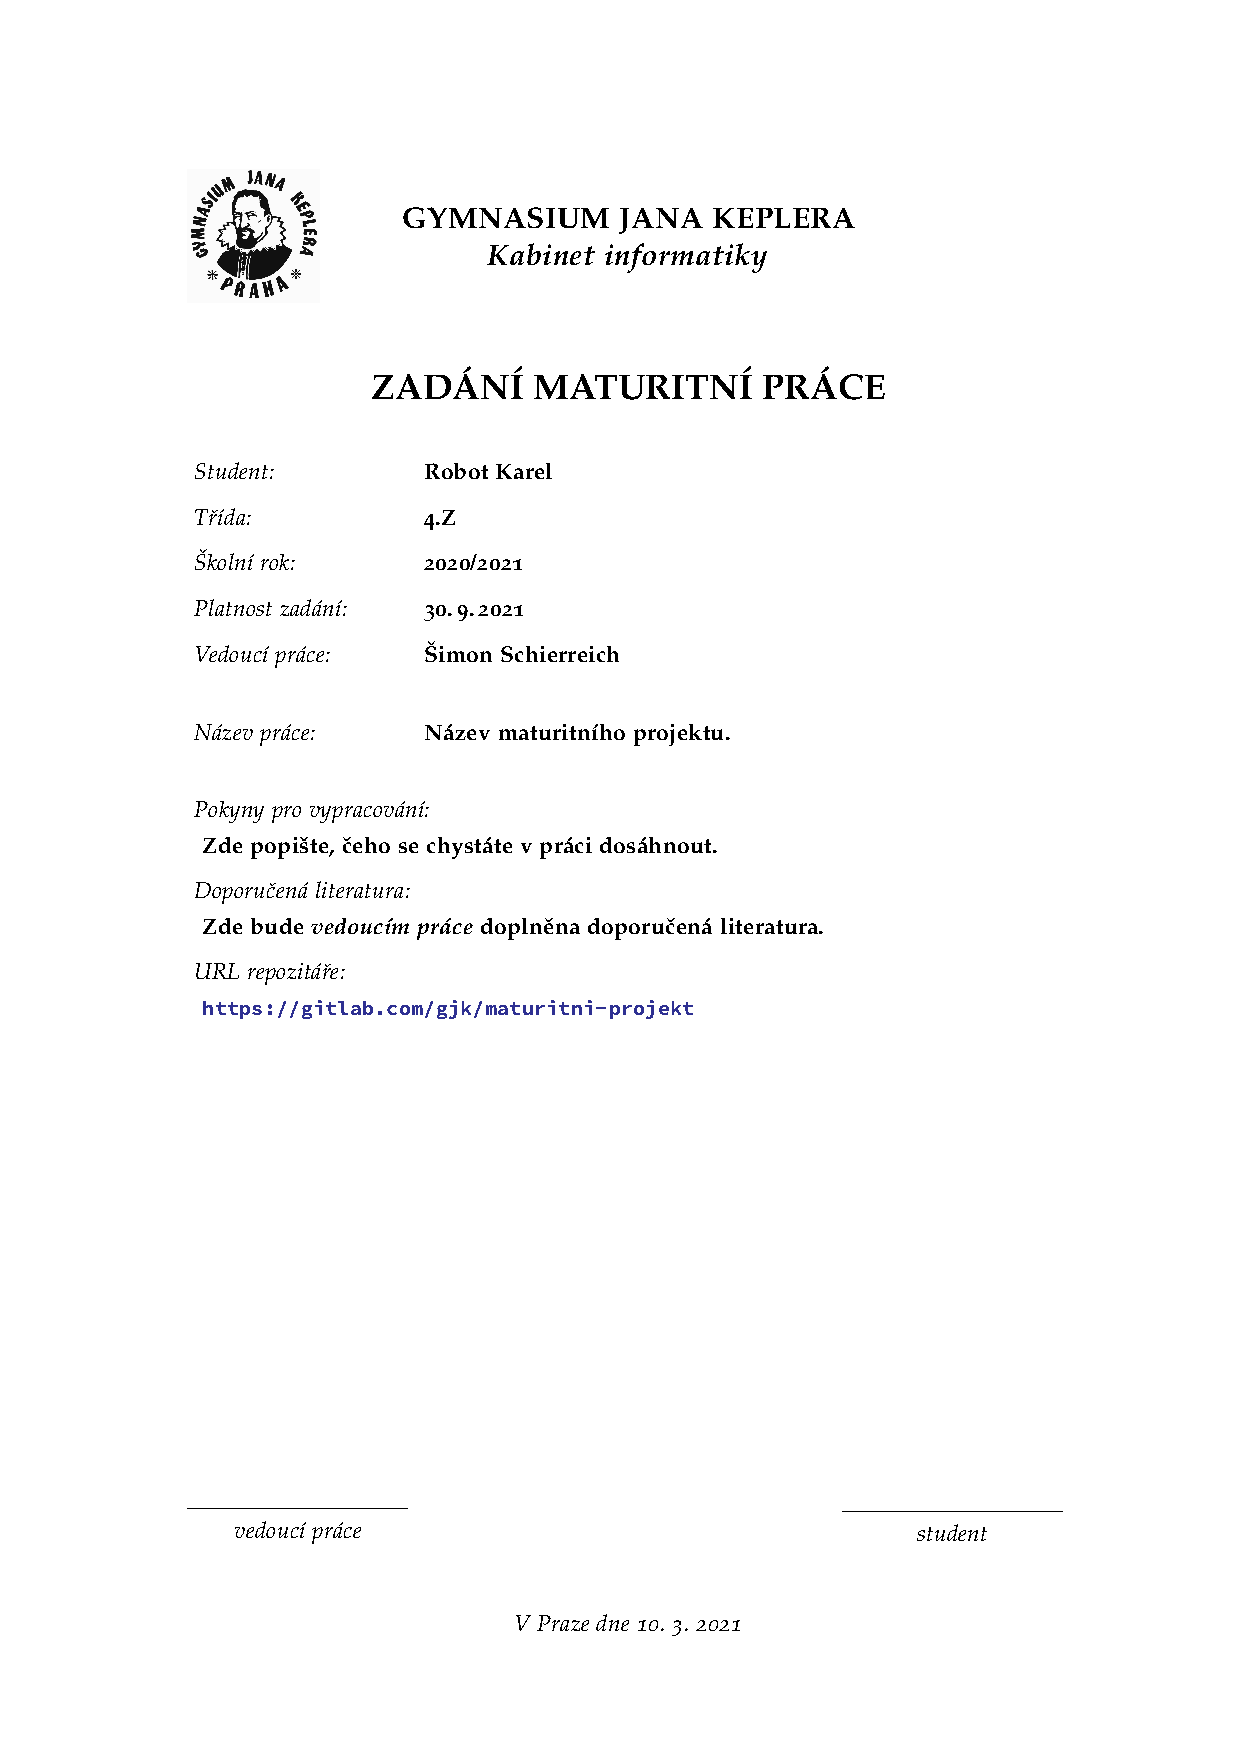
\includepdf[]{zadani.pdf}


%%% Strana s čestným prohlášením k bakalářské práci

\hypersetup{pageanchor=true}
\cleardoublepage
\vspace*{\fill}
\section*{Prohlášení}
\noindent
\Prohlaseni

\vspace{2cm}
\noindent
V Praze dne \today
\hspace*{\fill}\small{\AutorPrace}
\vspace{1cm}

%%% Poděkování
\openright
\vspace*{\fill}
\section*{Poděkování}
\noindent
\Podekovani
\vspace{1cm}


%%% Povinná informační strana bakalářské práce
\openright
\section*{Abstrakt}
\noindent
\Abstrakt
\subsection*{Klíčová slova}
\noindent
\KlicovaSlova

\vfill

\section*{Abstract}
\noindent
\AbstraktEN
\subsection*{Keywords}
\noindent
\KlicovaSlovaEN

\openright
\pagenumbering{arabic}

% Obsah
\setcounter{tocdepth}{2}
\tableofcontents

\chapter{Teoretická část}
\pagestyle{fancy}

V době, kdy jsem vymýšlel, co bych mohl vytvořit jako svůj maturitní projekt, se v médiích probírala možnost nákupu nových stíhacích letounů pro českou armádu. Odhadem se uváděla celková částka 48 miliard Kč. Slyšel jsem mnoho názorů o tom, jak moc peněz to je a že by bylo lepší peníze investovat jinam. Zamyslel jsem se tedy nad tím, kde stát peníze získává a za co je pak utrácí. V souvislosti s tím mě napadlo, kolik vlastně člověk sám odvede na daních do státního rozpočtu a jak by se tedy podílel na investicích a výdajích. 

Rozhodl jsem se tedy, že jako svůj maturitní projekt vytvořím webovou kalkulačku, která by se zabývala problematikou státního rozpočtu. Vytvořil jsem si představu, že uživatel do kolonek formuláře na webu zadá své příjmy a výdaje, kalkulačka údaje zpracuje a vypočítá z nich, jakou částku uživatel odvedl celkově za rok, který si vybere v nabídce, do státního rozpočtu. Uživatel by na stránce měl mít možnost prohlížet si údaje o státním rozpočtu z nabídky zpracovaných let. Dále jsem chtěl, aby kalkulčka zobrazila, prostřednitcvím jakých daní uživatel peníze státu odvedl. Tyto údaje by měly být společně v tabulce s celkovými státními příjmy. Vedle zobrazení státních výdajů jsem chtěl pak vypsat údaje o tom, jak se uživatelem odvedená částka rozpočítala na výdaje. Dále jsem na webu chtěl uvést některé konkrétní investice státu, kolik za ně stát utratil a jak se na nich podílel uživatel. Pro lepší celkovou funkcionalitu kalkulačky jsem se rozhodl, že kalkulačka musí mít i správu databáze údajů, které zobrazuje.

Z teoretické části jsem se tedy musel zaměřit především na daňový systém a údaje o státním rozpočtu. K tomu jsem také musel dohledat konkrétní investice státu a všechny tyto části spojit funkčně do sebe. Pro vytvoření funkční kalkulačky jsem tedy potřeboval získat údaje o státním rozpočtu za vybrané roky, údaje o konkrétních investicích, od uživatele přijmout údaje o jeho příjmech a výdajích a podle pravidel daňového systému vypočítat jeho podíl, který by pak kalkulačka rozložila mezi jednotlivé výdaje a investice.

\section{Státní rozpočet}

Svoji teoretickou analýzu jsem začal hledáním údajů o státním rozpočtu. Stát musí být v těchto záležitostech transparentní, a tak na webu ministerstva financí jsou k dispozici tabulky plnění státního rozpočtu, které uvádí jednotlivé důležité položky příjmů a výdajů státního rozpočtu. U každé položky je uvedeno, jaká hodnota se pro daný rok očekávala a jaká finálně hodnota skutečně byla. Já jsem samozřejmě pracoval se skutečnými hodnotami, aby kalkulačka byla přesnější. Rozhodl jsem se pro práci s údaji z let 2020, 2021 a 2022, protože v době dokončení projektu mají již vyplněné skutečné údaje. Počítal jsem s tím, že v rámci správy databáze bude pak možné přidat údaje i pro jiné roky.

Tyto údaje jsem si potřeboval pouze přepsat do databáze. Zpočátku jsem se potýkal s tím, že v souboru s údaji bylo více tabulek a uváděly různé příjmy. Na internetu jsem však poté dohledal, že existuje rozpočtové určení daní. Částka, kterou daňový poplatník odvede na daních, nemíří pouze do státního rozpočtu, ale dělí se. Část putuje do rozpočtu obcí, část do krajských rozpočtů a teprve zbytek skončí ve státním rozpočtu. Některé daně se dokonce odvádí pouze do obecních a krajských rozpočtů. Veřejné zdravotní pojištění se také nepočítá do příjmů státního rozpočtu. Pochopil jsem tedy, že do databáze si potřebuji vypsat údaje z tabulky, která zohledňuje opravdu pouze příjmy státního rozpočtu a ne celkové daňové příjmy.

\section{Konkrétní státní investice}

Vedle údajů o státním rozpočtu jsem také potřeboval získat příklady konkrétních investic a jejich náklady. Myslím si, že pro uživatele jsou snadno představitelnější a pochopitelnější konkrétní investice (např. nákup stíhacích letounů nebo dostavba Pražského okruhu) než obecné pojmy státních výdajů (např. neinvestiční transfery rozpočtům územní úrovně nebo ostatní běžné výdaje). Velmi dobře mi v tomto ohledu pomohl národní investiční plán na roky 2020 až 2050. Plán jsem prošel a vybral jsem si z něj důležité a velké investice, které jsem zapsal do databáze. Samozřejmě je možné přidávat další investice z plánu skrze správu databáze aplikace.

Při vybírání investic z plánu jsem si ale uvědomil problém složitosti výpočtu podílu jednotlivce na těchto investicích. Investice se většinou realizují mnoho let a není jasné, jakým přesným způsobem je stát financuje. Moje aplikace pracuje vždy s údaji za jeden rok, a i když z celkových výdajů státního rozpočtu vím, kolik putovalo na investice, tak nevím, kolik na jaké. Rozhodl jsem se tedy, že pro výpočet budu vycházet z předpokladu, že investice se celá realizovala a zaplatila pouze v roce, pro který si uživatel počítá své odvody a zobrazuje údaje o státním rozpočtu. U konkrétní investice by se tak zobrazil procentuální podíl na celkové částce, která za daný rok mířila na investice a podle toho částka, jakou by se uživatel podílel. Nejedná se tak o reálnou částku, ale i tak poskytuje představu o nákladnosti investice a velikosti podílu uživatele aplikace.

\section{Výpočet celkové odvedené částky na daních}

S již získanými obecnými informacemi o státních rozpočtech jsem se mohl zaměřit přímo na jednotlivce. Částku, kterou odvede do státního rozpočtu, musím určit z údajů, které mi poskytne. Potřeboval jsem si tedy rozmyslet, které údaje pro výpočet potřebuji od uživatele požadovat. Zaměřil jsem se tedy na státní příjmy a podíval se, které daně přináší peníze do rozpočtu. Z těch jsem si vybral ty, na kterých se podílí jednotlivec sám - DPH, daň z příjmu fyzických osob, pojistné na sociální zabezpečení, daň z hazardu a spotřební daň z paliva, tabáku a alkoholu. Podle toho jsem si určil, jaké údaje od uživatele budu požadovat, abych konkrétní daň vypočítal.

\subsection{DPH}

DPH se dělí podle procentuálního odvodu do tří kategorií - základní sazba, první snížená sazba a druhá snížená sazba. V druhé snížené sazbě se odvádí daň ve výši 10\%, a to především z vodného a stočného, nákupu knih, hudby, léků a z ubytovacích služeb. V první snížené sazbě to je 15\% a vyměřuje se pro potraviny a gastronomické služby, veřejnou dopravu a léčební pomůcky. Základní sazba je 21\% a vztahuje se na všechny ostatní nákupy a útraty. Od uživatele tedy potřebuji zjistit, kolik průměrné měsíčně utratí za dané kategorie.

\subsection{Daň z příjmu}

Daň z příjmu fyzických osob se dnes vypočítává z hrubého příjmu. Z hrubého příjmu tvoří 15\%. Výpočet probíhá tak, že si spočítáme 15\% z hrubého příjmu a odečteme od toho slevu na poplatníka - 2570 Kč měsíčně. Do roku 2020 se daň vypočítávala ze superhrubé mzdy - 15\% z 1,338 násobku hrubé mzdy. Pokud si poplatník nárokuje slevu na dítě, odečte se i ta. Sleva na první dítě je 15 204 Kč za rok, na druhé 22 320 Kč za rok a na každé další 27 840 Kč za rok. Dříve byl maximální součet omezen na 60 300 Kč za rok, od roku 2022 sleva na děti nemá horní hranici. Ze slevy na děti je možné vyměřit daňový bonus. Tedy pokud sleva na děti převyšuje daň z příjmů, stát musí uhradit daňovému plátci rozdíl. V extrémních případech může stát díky slevě na děti zaplatit jednotlivci více, než by jinak jednotlivec celkově odvedl do státního rozpočtu. Na slevu má nárok pouze jeden z rodičů. K dani z příjmu patří ještě daň z kapitálových příjmů. To je také 15\%, ale vyměřuje se pouze, pokud za rok plátce zaznamená zisk z kapitálových příjmů vyšší než 100 000 Kč. Pro výpočet musí uživatel zadat svůj hrubý příjem, počet dětí, pokud na ně uplatňuje slevu, a kapitálové příjmy.

\subsection{Sociální pojištění}

Při výpočtu odvodu na sociální pojištění záleží na tom, jestli je uživatel zaměstnanec nebo OSVČ. Výpočet se podle toho liší. V případě OSVČ jsem se rozhodl částku nepočítat, protože nevím, z jakého vyměřovacího základu si ji uživatel počítá. Po uživateli, který je OSVČ, tedy požaduji, aby vyplnil kolonku s tím, kolik si na pojištění platí. Stejně tak požaduji, aby kolonku vyplnili ti, co pracují jako zaměstnanci, ale na zkrácený úvazek. Opět nevím, z čeho bych daň vypočítal. Pro klasické zaměstnance je to pak jednoduché. Zaměstnanec  na sociální pojištění sám odvádí 6,5\% ze své hrubé mzdy a k tomu za něj zaměstnavatel odvádí ještě 24,8\% z hrubé mzdy. Ve své aplikaci zohledňuji i peníze odvedené zaměstnavatelem, protože je také vnímám jako odměnu za práci zaměstnance.

\subsection{Spotřební daně a daň z hazardu}

Daň z hazardu je 23\%, spotřební daň z paliv je v průměru 11,5 Kč/l, spotřební daň z piva je 0,32 Kč/l, spotřební daň z lihovin je 322,5 Kč na litr ethanolu a spotřební daň za jednu cigaretu je 2,9 Kč. Uživatel tedy do kolonek zadá průměrnou částku, kterou prohraje na hazardu, kolik utratí za paliva, kolik vypije piva a lihovin a kolik vykouří cigaret za měsíc.

\subsection{Finální částka}

V instrukcích jsem upřesnil, že uživatelé mají do každé kolonky vyplnit průměrnou měsíční hodnotu údaje. Pomocí výše uvedených procentuálních sazeb kalkulačka spočítá, kolik peněz uživatel odvedl na daních za vybrané položky a samozřejmě to vynásobí dvanácti, aby výsledkem byl údaj za celý rok. U vybraných daní také zohlední rozpočtové určení daní. Z prostředků odvedených prostřednictvím DPH a daně z příjmu fyzických osob míří do státního rozpočtu pouze 64,38\%. U daně z hazardu je to 70\%. Výsledkem výpočtů je celková částka, kterou uživatel za rok odvedl do státního rozpočtu.

\section{Rozbor uplatnění odvedené částky}

Pokud má aplikace údaje o státním rozpočtu, konkrétních investicích a částku zaplacenou uživatelem na daních, může začít zobrazovat informace o uplatnění odvedených peněz. V úvodu teoretické analýzy jsem uvedl, co by kalkulačka měla zobrazovat - kolik prostřednictvím jakých daní uživatel odvedl do rozpočtu, jak se peníze přerozdělily na výdaje a jak by se uživatel hypoteticky podílel na konkrétních investicích.

\subsection{Analýza kompozice odvedené částky}

Uživateli se vedle položek státních příjmů zobrazí, kolika korunami se na této položce podílel. Výpočet odpovídá postupům, které jsem uvedl u výpočtu celkové částky. Pouze zde aplikace zobrazuje částky odvedené na jednotlivých daní a nesčítá je.

\subsection{Analýza reálného uplatnění odvedené částky}

Uživateli se vedle položek státních výdajů zobrazí, kolika korunami se na této položce podílel. Výpočet je velmi jednoduchý. U každé položky aplikace vypočítá, jaký podíl položka tvoří z celkových výdajů. Toto procento aplikuje pak na částku odvedenou uživatelem na daních. Částka se tedy rozpočítá mezi jednotlivé položky ve stejném poměru, jako je to u celkových státních výdajů.

\subsection{Hypotetický podíl na konkrétních investicích}

Zde kalkulačka vezme celkové náklady konkrétní investice a spočítá, jaký procentuální podíl by náklady tvořily z peněz vyčleněných na investice za daný rok. Korunový podíl uživatele je výsledkem násobení vypočteného procenta a částky, kterou uživatel odvedl na daních a putovala na investice. V sekci 1.2 vysvětluji nepřesnosti tohoto výpočtu.

\chapter{Implementace}

\section{Zvolené technologie}
Na implementaci projektu jsem zvolil následující technologie:

\begin{itemize}
  \item Programovací jazyk Python
  \item Programovací jazyk JavaScript
  \item Flask framework
  \item AlpineJS framework
  \item PicoCSS styly
  \item PocketBase
\end{itemize}

\subsection{Programovací jazyk Python}
Python jsem zvolil z více důvodů. Mé dva hlavní důvody byly praktičnost a technický aspekt. Python je
pro mě praktický, protože jsem se s ním dříve setkal při výuce informatiky, a tak jsem se spoléhal, že
si jej připomenu a bude jednodušší pro mě jej používat, než abych se učil nový jazyk, se kterým vůbec nemám
zkušenosti.

Technický aspekt, proč jsem zvolil Python, je kvůli přesnosti jeho matematiky. Na semináři jsme se učili o
standardu IEEE-754 a jeho nepřesnostech, a podle mého vyhledávání na internetu se tato čísla používají jako
výchozí čísla s desetinnou čárkou ve většině populárních programovacích jazycích. Python používá čísla s
neomezenou přesností, což mi pomáhá dělat přesnější výpočty. Vím, že pro ostatní programovací jazyky existují
knihovny, které přidávají další číselné typy, ale to by byla komplexita navíc. Je mi také jasné, že čísla
s neomezenou přesností jsou mnohem méně výkonné, než IEEE-754, ale pro účely mého projektu není výkon kritickým
aspektem.

\subsection{Programovací jazyk JavaScript}
Jednou z mých obecných motivací při volbě použitých technologií byla jednoduchost. Nechtěl jsem používat
nástroje navíc a zbytečně velké technologie. Nejsem sice odborníkem na tuto problematiku, ale NodeJS a další
webové runtimy mi připadaly jako přehnané pro můj projekt. S JavaScriptem jsem se také setkal na školní informatice.
Z těchto důvodů jsem rozhodl zvolit JavaScript, i když si jsem vědom některých jeho slabin a nepředvídatelného
chování.

S použitím JavaScriptu přímo v prohlížeči, bez žádného mezikroku jako NodeJS, Bun, nebo Deno, ve spolupráci
s frameworkem AlpineJS se mi podařilo mít na frontendu pouze jeden jazyk a pouze
jednu malou knihovnu jako závislost.

\subsection{Flask framework}
V Pythonu jsem slyšel o dvou knihovnách pro tvorbu webových aplikací - Flask a Django. Django se mi zdálo
jako moc složité pro moje účely, a to byl hlavní důvod, proč jsem zvolil Flask. Pro Flask také existuje
kurz na Codecademy, který má velký překryv s dalšími kurzy, které jsem splnil v přípravě na maturitní projekt,
volba Flasku mi tedy ušetřila čas.

\subsection{AlpineJS framework}
O této knihovně jsem se dozvěděl z youtube videa na kanálu \emph{Fireship}. Líbilo se mi, že s ním můžu
vepisovat chování rovnou do HTML, bez toho, aniž bych musel psát velké množství JavaScriptu. AlpineJS se
dá do libovolné stránky vložit pomocí \emph{<script>} tagu, díky čemuž jsem se opět vyhnul studia NodeJS
a dalších, složitějších technologií.

Přístup AlpineJS mi připadá vizuálně přehledný a, přestože se jedná relativně malý framework, neměl jsem
pocit, že by mi v něm chyběla nějaká funkcionalita.

Způsob přemýšlení, který AlpineJS vyžaduje, byl pro mě ze začátku nezvyklý. V Alpine se většina akcí a interaktivity
definuje pomocí atributů na HTML.

Například:

\begin{verbatim}
<section
	class="user_buttons"
	x-data="{ is_logged: false, is_admin: false }"
	x-init="
		is_logged = window.localStorage.getItem('pocketbase_auth') !== null;
		is_admin = window.localStorage.getItem('pocketbase_auth') !== null;
	"
>
    <a
    	role="button"
    	href="/login"
    	x-show="!is_logged"
    >
    	Login
    </a>
    <a
    	role="button"
    	href="/admin"
    	x-show="is_logged && is_admin"
    >
        Admin
    </a>
    <a
        role="button"
        href="#"
        x-show="is_logged"
        x-on:click.prevent="pb_logout(client); is_logged = false;"
    >
    	Logout
    </a>
</section>
\end{verbatim}

Základní proces vývoje je takový, že si definuji na HTML prvcích, které mají být interaktivní,
atribut \textbf{x-data}, ve kterém mám uložené v JavaScriptové objektové syntaxi proměnné patřící
k tomuto prvku.

K těmto proměnným se pak mohu odkazovat v jiných atributech na tomto prvku a na prvcích, které jsou
potomky tohoto prvku.

Dalším krokem je přidávání atributů jako \textbf{x-show} (podmínky, za kterých se má prvek zobrazovat)
a \textbf{x-if}(podmínky, za kterých má prvek vůbec existovat, a tam, kde potřebuji zobrazit text
nějaké proměnné, parametr \textbf{x-text}.

Například, zde je textový \emph{input} a výpis textu, který je v něm napsaný:

\begin{verbatim}
<div x-data="{ vstup: '' }">
   <p x-text="vstup"></p>
   <input type="text" x-model="vstup">
</div>
\end{verbatim}

AlpineJS je reaktivní, takže každá změna v inputu se automaticky zpropaguje skrz proměnnou \textbf{vstup}.

To mě vede k posledním dvěma atributům, které byly klíčové na straně AlpineJS. Atribut \textbf{x-init}
diktuje kód, který se spustí, když se prvek poprvé načte, a atribut \textbf{x-effect} se spustí, když
se stránka načte, a pokaždé, když dojde ke změnám v reaktivních proměnných definovaných v \textbf{x-data},
které jsou v kódu tohoto atributu zmíněny.

V některých případech se hodí nemít jednotný \textbf{x-effect}, protože tím může docházet k vykonávání
zbytečné (nebo i nežádoucí) práce. Pro tyto situace je možné použít \emph{kouzelnou funkci} (dle terminologie
AlpineJS) \textbf{\$watch('jmeno\_promenne', hodnota => akce)}, která umožňuje reagovat na individuální
změny proměnných.

Tyto atributy používám k volání svého JavaScriptového kódu, který mám rozčleněný do dalších souborů.

\subsection{PicoCSS}

PicoCSS jsem zvolil jako minimalistický CSS framework. Nechtěl jsem všechny styly psát ručně, protože
nejsem odborník na design a typografii, ale nechtěl jsem importovat velké a složité frameworky jako
Bootstrap, které bych se musel učit. O PicoCSS jsem se také dozvěděl z YouTube videa. Kromě jeho jednoduchosti
a malé velikosti mě zaujalo především to, že nevyžaduje, abych všude psal CSS třídy a učil se, jak se
jmenují. PicoCSS definuje styly pro HTML elementy a používá další kontextové informace k identifikaci,
jak by měl být daný prvek zobrazen.

Například zobrazení karty, kterou jde skrýt pod její nadpis, vypadá takto:

\begin{verbatim}
<details>
  <summary>Nadpis</summary>
  <p>obsah</p>
  <p>atd.</p>
  <p>atd.</p>
</details>
\end{verbatim}

Tuto funkcionalitu jsem používal na formátování svého layoutu způsobem, který mi připadal velmi praktický.
Nevýhodou tohoto způsobu je však to, že zneužívá HTML5 sémantické prvky, které pak nemají nutně úplně logickou
strukturu.

Například toto je sekce, kde zobrazuji formulář, příjmy a výdaje státu. Potřeboval jsem vzhled, který
je nadefinovaný na tagu \textbf{<article>}, i když vím, že ani jeden z těchto prvků není článkem:

\begin{verbatim}
<section class="main" x-data>
    <article class="calc-form form">
       ...
    </article>
    <article class="prijmy" x-data>
       ...
    </article>
    <article class="vydaje" x-data>
       ...
    </article>
</section>
\end{verbatim}

Nemyslím si, že by to toto byl zas tak pádný nedostatek v případě mojí aplikace, protože se nejedná o
aplikaci určenou ke čtení nástroji, pro které jsou sémantické tagy důležité. Kdyby můj projekt spravoval
například blogy, novinové články nebo odborné příspěvky, bylo by správné použití sématických tagů
mnohem důležitější.

Nezvyklým aspektem pro mě bylo rozlišování CSS stylů na základě parametrů jako \textbf{role="button"} nebo
\textbf{aria-busy="true"}.

\subsection{PocketBase}
Ještě než jsem se pustil do implementace projektu mi bylo jasné, že budu potřebovat databázi. Z hodin
informatiky a semináře jsem věděl o databá S kbdzích jako je SQLite nebo PostgreSQL, ale připadaly mi moc
složité. Rozhodl jsem se proto najít nějaké řešení, které by bylo jednodušší, a přineslo by mi nejen databázi
samotnou, ale i kvalitní podporu jak pro Python, tak pro Javascript, a pomohlo mi se správou uživatelů.
Slyšel jsem o projektu Firebase od Googlu, ale ten se mi zdál moc složitý, a nelíbila se mi myšlenka,
že by můj projekt závisel na Googlu.

Nakonec jsem, opět na Youtube kanálu Fireship, dozvěděl o projektu PocketBase. PocketBase má webové API,
pro které existuje JavaScriptový i Pythonový klient, má přehledné webové rozhraní, zabudovaný koncept uživatelů
a jejich správy a umožňuje mi specifikovat pravidla, tak abych měl jistotu, že k databázi mohu přistupovat
i z frontendu bez toho, aniž bych se vystavil riziku, že mi některý z uživatelů databázi zlomyslně vymaže.

Pro jazyky JavaScript a Dart generuje PocketBase ukázky, jak provádět různé úkony na příslušné tabulce.
Například, u akce pro přidání nové investice, vygeneruje webové rozhraní toto:

\begin{verbatim}
import PocketBase from 'pocketbase';

const pb = new PocketBase('https://pocketbase.gjk.cat');

...

// example create data
const data = {
    "start_year": 123,
    "name": "test",
    "cost": 123
};

const record = await pb.collection('investments').create(data);
\end{verbatim}

Díky těmto ukázkám jsem se v PocketBase rychle zorientoval. Velmi užitečné bylo také nastavení pravidel,
které používám u uživatelských investic:

\begin{verbatim}
# create action - custom rule
user_id = @request.auth.id

# update action - custom rule
user_id = @request.auth.id

# delete action - custom rule
user_id = @request.auth.id
\end{verbatim}

Díky těmto pravidlům mám jistotu, že každý normální uživatel může přidávat, upravovat a odebírat pouze svoje
investice, a nepotřebuji tuto akci provádět skrze svůj Flaskový backend, který by data a přístupy validoval
manuálně.

PocketBase má zabudovaný webserver a jde v něm vyvíjet plnohodnotné aplikace pomocí rozšíření napsaných
v jazyce Go. Protože však Flask vyžaduje WSGI server a já neumím Go, nemohl jsem toto využít.

Domnívám se, že pro znalce Go by bylo možné celou aplikaci napsat bez jakéhokoliv separátního backendu,
a mít celý projekt jako jeden monolitický celek spravovaný PocketBasem.

Velmi užitečnou funkcí na PocketBase je také \emph{Request log}, díky kterému jsem mohl zkoumat, proč
něco, co zkouším, nefunguje. Když jsem se snažil přijít na to, jak správně filtrovat v databázi, vyhledávač
požadavků byl další ergonomickou funkcí PocketBase.

PocketBase také obsahuje integraci pro přihlašování skrze služby jako je Google účet, Facebook účet,
Gitlab, nebo Twitch, ale do těchto integrací jsem se nepouštěl.

Je nutné podotknout, že PocketBase je primárně interaktivní nástroj, schéma databáze jsem si musel
manuálně exportovat do JSON souboru, import musí být také ruční.

\section{Postup implementace}

Pro mojí práci jsou klíčová data získaná od státu. Bez správných dat a správné organizace těchto dat
bych nemohl provádět výpočty. Začal jsem tedy svůj postup od databáze tvorbou jednotlivých tabulek
a naplňováním těchto tabulek daty.

Všechny tabulky prošly několika verzemi, než jsem s nimi byl spokojený (a stejně jsem musel ještě
během vývoje zbytku aplikace dělat v tabulkách drobné úpravy). Tabulku na uživatelské investice
jsem přidal až na závěr.

Když jsem byl spokojený s daty, ze kterých moje aplikace vychází, vytvořil jsem nový Flaskový projekt.
Pro základní nastavení projektu jsem použil nástroj Nix, o kterém jsem se dozvěděl díky bratrovi, který
mi doporučil a nainstaloval NixOS jakožto \emph{"nerozbitný Linux"}. Je nutné podotknout, že Nix a NixOS
není to samé. Termín Nix označuje dvě věci - Nix jazyk a Nix balíčkovač, který je na tom jazyce postavený.
NixOS je distribuce postavené na Nixu - balíčkovači. Nix jakožto balíčkovač, build systém a nástroj pro
vytváření konzistentních prostředí a konfigurace není nijak závislý na NixOS a funguje na libovolné
linuxové distribuci (i macOS v omezené míře), podobně jako Docker.

Rozdíl mezi Dockerem a Nixem je ten, že Docker je imperativní, psaní Dockerfile souborů můžeme přirovnat
k psaní instrukcí v receptu do kuchařky, kdežto Nix je deklarativní, specifikuji, co potřebuji, a to mám.

Pro účely mého projektu mi stačilo napsat pouze soubor \emph{shell.nix}, který mi vytvoří prostředí,
které má potřebné závislosti, nakonfigurované proměnné prostředí a vstoupí do virtuálního Python prostředí.

Zde je moje Nix konfigurace pro tento projekt:
\begin{verbatim}
{ pkgs ? import <nixpkgs> { } }:

pkgs.mkShell {
  buildInputs = [
    pkgs.coreutils-full
    pkgs.python3Full
    pkgs.python3.pkgs.virtualenv
    pkgs.python310Packages.waitress
    pkgs.pocketbase
  ];
  shellHook = ''
    virtualenv -p python3 env
    source env/bin/activate
    pip install -r requirements.txt
  '';
  FLASK_APP = "src/main.py";
  POCKETBASE_URL = "https://pocketbase.gjk.cat/";
}
\end{verbatim}

Pole \emph{buildInputs} specifikuje, jaké programy potřebuji mít v prostředí, \emph{shellHook} co se má
stát při spuštění tohoto shellu, a ostatní jsou proměnné prostředí.


V této době jsem ještě neměl dokončený online kurz Flasku, tak jsem tento framework teprve zkoušel. První
endpoint vracel pouze string \emph{"ahoj"}.

Později jsem přidal knihovnu pro PocketBase a začal psát soubor s matematickými funkcemi pro výpočty
jednotlivých statistik (\emph{tax\_math.py}). Vytvořil jsem několik endpointů, které prakticky pouze
přeposílaly data z PocketBase. Těmto endpointům jsem se teoreticky mohl vyhnout, ale vzhledem k tomu,
že jsem data z tabulek potřeboval číst i ve Flaskové aplikaci, jsem je vytvořil a volal je rovnou ve
Flasku, místo toho, abych si je posílal přes frontend.

Moje teze je, že tento přístup je rychlejší a efektivnější, když se PocketBase i Flask nachází na stejném
stroji. Tyto endpointy používám i na frontendu, když už jsem je měl připravené. Pro vnitřní použití ve
Flasku jsem je ale musel rozdělit na dvě funkce, kdy jedna získává data a druhá je flaskovým endpointem,
který je posílá jako odpověď.

Například, zde je tento pár pro získání dat pro rozpočet na daný rok:

\begin{verbatim}
def fetch_rozpocet_na_rok(rok):
    rozpocty = fetch_all_for_table('budgets')

    spravny_rozpocet =
      next(rozpocet for rozpocet in rozpocty if rozpocet.year == rok)
    return Budget(spravny_rozpocet)

@app.route("/rozpocet/<int:rok>")
def rozpocet_na_rok(rok):
    rozpocet = fetch_rozpocet_na_rok(rok)
    return rozpocet.to_json()
\end{verbatim}

Kvůli konverzi na JSON jsem si modely opsal do Pythonu, a naimplementoval na nich manuální převod
následujícím způsobem:

\begin{verbatim}
from flask import jsonify

class Budget:
    def __init__(self, record):
        print(record)
        self.year = record.year
        self.total_income = record.total_income
        self.total_expense = record.total_expense
        self.vat = record.vat
        self.consumer_taxes = record.consumer_taxes
        self.income_tax_individual = record.income_tax_individual
        self.income_tax_company = record.income_tax_company
        self.mandatory_social_insurance = record.mandatory_social_insurance
        self.other_tax = record.other_tax
        self.other_nontax_income = record.other_nontax_income
        self.consumer_tax_oils = record.consumer_tax_oils
        self.consumer_tax_tobacco = record.consumer_tax_tobacco
        self.consumer_tax_solar_energy = record.consumer_tax_solar_energy
        self.trash_fees = record.trash_fees
        self.gambling_tax = record.gambling_tax
        self.income_from_eu = record.income_from_eu
        self.income_connected_with_eu = record.income_connected_with_eu
        print(dir(self))         # debugging
        print(self.total_income) #

    def to_json(self):
        return jsonify(
            year=self.year,
            total_income=self.total_income,
            total_expense=self.total_expense,
            vat=self.vat,
            consumer_taxes=self.consumer_taxes,
            income_tax_individual=self.income_tax_individual,
            income_tax_company=self.income_tax_company,
            mandatory_social_insurance=self.mandatory_social_insurance,
            other_tax=self.other_tax,
            other_nontax_income=self.other_nontax_income,
            consumer_tax_oils=self.consumer_tax_oils,
            consumer_tax_tobacco=self.consumer_tax_tobacco,
            consumer_tax_solar_energy=self.consumer_tax_solar_energy,
            trash_fees=self.trash_fees,
            gambling_tax=self.gambling_tax,
            income_from_eu=self.income_from_eu,
            income_connected_with_eu=self.income_connected_with_eu,
        )
\end{verbatim}

Uznávám, že tento způsob je trochu repetitivní, a že může docházet k chybám kvůli překlepům. Složitější řešení,
která jsem na internetu potkal, mi ale připadala nepřehledná pro tuto aplikaci.

Tyto základní endpointy jsem testoval pomocí programu \textbf{cURL}, v této chvíli neexistovalo ještě konkrétní
spojení frontendu a backendu.

Posléze jsem začal realizovat i vzhled frontendu. Nejdřív jsem psal pouze HTML, framework PicoCSS jsem přidal
později, a AlpineJS jsem doopravdy začal používat až když jsem měl hlavní prvky vzhledu svojí aplikace.

Můj první experiment s frameworkem AlpineJS bylo dynamické zobrazování roku v textu footeru stránky:

\begin{verbatim}
<footer>
    Tomáš Hozda © <span x-text="new Date().getFullYear()"></span>
</footer>
\end{verbatim}

Finální vzhled vzniknul částečně jako bug. Rozložení příjmů, výdajů a formuláře na ůdaje uživatele měly být
tři rovnocené sloupce stejné barvy, ale kvůli špatně uzavřeným HTML tagům byl prostřední sloupec šedivý a zasunutý
za těmi postraními. Tento vzhled se mi zalíbil, tak jsem se pro něj po opravě této chyby rozhodl.

Nejnovější koncepty v CSS pro mě byly \emph{grid layout} a \emph{flexbox}. Flexbox jsem použil ve dvou případech:

\begin{itemize}
  \item Pro zobrazování více prvků najednou tak, aby se poskládaly správně na obrazovku (např. dlaždice s investicemi)
  \item Pro centrování prvků v jejich rodičích
\end{itemize}

Příklad prvního použití u dlaždic investic:

\begin{verbatim}
flexperiment {
    display: flex;
    flex-flow: row wrap;
    justify-content: center;
    width: 100vw;
    margin-left: calc((100vw - 100%) / -2);
    margin-right: calc((100vw - 100%) / -2);
}

.flexperiment article {
    flex-grow: 0;
}
\end{verbatim}

A centrování prvků:

\begin{verbatim}
.center-example {
    display: flex;
    align-items: center;
    justify-content: center;
}
\end{verbatim}

Intenzivní použití AlpineJS bylo až ke konci práce, když jsem potřeboval adekvátně spojit frontend a backend.
V některých případech jsem narazil na nekonzistentní chování v AlpineJS. Zmíním dva příklady.

Pomocí atributu \textbf{x-for} na HTML tagu \emph{<template>} je možné generovat prvky pro každý element
pole. Používám jej vždy při zobrazování prvků nějaké tabulky z PocketBase. Když dochází k přidávání a odebírání
elementů v poli bez toho, aniž by bylo vytvořeno nové pole, AlpineJS nedokáže poznat, o které prvky se jedná,
a dochází k nezobrazování nebo duplikovanému zobrazení prvků.

V těchto případech je zapotřebí specifikovat nějakou vlastnost prvků pole jako klíč:

\begin{verbatim}
<template x-for="data in budgets" :key="data.id">
  ...
</template>
\end{verbatim}

Druhá nekonzistence, se kterou jsem se potýkal, je reaktivnost v atributech \textbf{x-effect}. Když je kód
moc komplexní a figuruje v něm mnoho reaktivních proměnný, tak je možné, že AlpineJS nedetekuje všechny
odkazy a nepouští kód ve všechny správné momenty. Tento problém jsem ve všech případech vyřešil pomocí
výše zmíněné \textbf{\$watch()} funkce sledováním jednotlivých proměnných.


\chapter{Technická dokumentace}

\section{Požadavky}
Projekt je možné zprovoznit dvěma způsoby, za použití Nixu a bez něj. Postup s použitím Nixu je jednodušší a spolehlivější,
ale je použitelný pouze na Linuxových distribucích (a případně Macu), protože pro Windows nemá Nix podporu.

S Nixem jsou závislosti pro spuštění následující:

\begin{itemize}
  \item Rozumná Linuxová distribuce (nebo MacOS)
  \item \href{https://nixos.org/}{Nix}
  \item \href{}{Git}
\end{itemize}

V případě postupu bez Nixu je možné použít i Windows, ale je zapotřebí explicitně nainstalovat více závislostí:

\begin{itemize}
\item Python 3 (projekt byl vyvíjen s Pythonem 3.10.9, ale neměly by být problémy s kompatibilitou s novějšími verzemi)
\item PocketBase
\item \href{https://flask.palletsprojects.com/en/2.2.x/}{Flask}
\item \href{https://pypi.org/project/waitress/}{waitress} (na deployment)
\end{itemize}

Následující instrukce jsou pro Linuxové operační systémy, jakožto pro platformu, která se nejvíc hodí
na vývoj a provoz aplikací.

\subsection{Git}
Git by měl být předinstalovaný na většině distribucí. Pokud není, zpravidla je možné jej
nainstalovat pomocí balíčkovače systému:

\begin{verbatim}
# debianovité distribuce
sudo apt-get install git

# archovité distribuce
sudo pacman -S git

# void linux
sudo xbps-install -Sy git
\end{verbatim}

Pro zprovoznění maturitního projektu takhle git stačí, v praxi si však uživatel často bude potřebovat
nakonfigurovat jméno, email, a SSH klíč.
 S kbd
\subsection{Nix}
Nix je možné nainstalovat pomocí balíčkovače na vaší distribuci, například:

\begin{verbatim}
# debianovité distribuce
sudo apt-get install nix

# archovité distribuce
sudo pacman -S nix

# void linux
sudo xbps-install -Sy nix
\end{verbatim}

Doporučený je ale způsob z webové stránky Nixu\footnote{\url{https://nixos.org}}, který nainstaluje
Nix přes Nix:
\begin{verbatim}
$ sh <(curl -L https://nixos.org/nix/install) --daemon
\end{verbatim}

Aby uživatelé nepotřebovali na provoz Nixu práva superuživatele, vyplatí se pustit nixového démona:
\begin{verbatim}
# nix-daemon
\end{verbatim}

Každý uživatel si potom musí nastavit proměnnou  {\bf NIX\_REMOTE} na hodnotu {\bf daemon}:

\begin{verbatim}
echo 'export NIX_REMOTE=daemon' >> $HOME/.bashrc #nebo jinak pro jiné shelly
\end{verbatim}

Funkčnost Nixu můžeme ověřit například následujícím způsobem:

\begin{verbatim}
$ nix-shell -p neo-cowsay
[nix-shell:~]$ cowsay kůň
 _____
< kůň >
 -----
        \   ^__^
         \  (oo)\_______
            (__)\       )\/\
                ||----w |
                ||     ||
\end{verbatim}

\subsection{Python}
Programovací jazyk Python je, podobně jako Git, na většině distribucí předinstalován. V případě,
že tomu tak není, můžeme se ve většině případů opět spolehnout na nativní balíčkovač systému: 

\begin{verbatim}
# debianovité distribuce
sudo apt-get install python

# archovité distribuce
sudo pacman -S python

# void linux
sudo xbps-install -Sy python
\end{verbatim}

Backend aplikace neobsahuje žádný složitý Python, kde by připadala v úvahu citlivost na verzi Pythonu.
Projekt byl vyvinut s Pythonem 3.10.9, tuto verzi a každou novější můžeme považovat za jistotu.

Je důležité podotknout, že některé instalace Pythonu jsou spíš minimalistické a neobsahují nástroje
jako \emph{pip} a \emph{venv/virtualenv}, které je potom potřeba doinstalovat separátně.

\subsection{PocketBase}
PocketBase je asi nejméně známý software, co je potřeba nainstalovat pro zprovoznění aplikace.
V případě, že nebude dostupný v balíčkovači linuxové distribuce, je zapotřebí jej nainstalovat
buď stažením archivu z webu projektu:

\url{https://pocketbase.io/docs/}

Nebo, v případě, že distribuce obsahuje Go buď nainstalované nebo v repozitáři balíčkovače:

\begin{verbatim}
go get github.com/pocketbase/pocketbase
\end{verbatim}

Pro práci s PocketBase je zapotřebí ještě nainstalovat Pythonovou PocketBase knihovnu.
Nejjednodušší je vytvořit virtuální prostředí a nainstalovat PocketBase pomocí \emph{pipu}
ze souboru \emph{requirements.txt}:

\begin{verbatim}
virtualenv -p python3 env
source env/bin/activate
pip install -r requirements.txt
\end{verbatim}

\subsection{Flask}
Podobně jako klientskou knihovnu PocketBase, je možné Flask nainstalovat ze souboru
\emph{requirements.txt} pomocí \emph{pipu}. Vzhledem k tomu, že použití Flasku v tomto
projektu není komplexní, měly by fungovat i verze z balíčkovače distribuce.

\subsection{waitress}
WSGI server \emph{waitress} je nutný nainstalovat pouze na produkční provoz aplikace,
pro vývoj a testování aplikace stačí server zabudovaný v příkazu \emph{flask run}. Program \emph{waitress} se dá nainstalovat z balíčkovače některých linuxových distribucí, nebo pomocí pipu:

\begin{verbatim}
pip install waitress
\end{verbatim}

\section{Instalace a spouštění}
Pro spuštění projektu je nejdříve potřeba naklonovat
repozitář:

\begin{verbatim}
git clone https://github.com/Tomdrs/statni_rozpocet
\end{verbatim}

Dobrovolným krokem je spustit lokální instanci PocketBase:

\begin{verbatim}
pocketbase serve
\end{verbatim}

Tato instance PocketBase bude prázdná. Postup pro naimportování
databázového schématu je následující:

\begin{enumerate}
  \item Otevřete v prohlížeči adresu \url{http://localhost:8090/_/}
  \item Vytvořte první admin účet podle instrukcí na obrazovce
  \item V kartě \emph{Settings} v sidebaru na levé straně naimportujte schéma ze souboru \emph{pb\_schema.json} v repozitáři
  \item Případně rozšiřte nebo upravte data v jednotlivých tabulkách
\end{enumerate}

Kromě lokální instance PocketBase je možné použít instanci na adrese \url{https://pocketbase.gjk.cat}.
Dalším krokem je nastavení proměnných prostředí:

\begin{verbatim}
export FLASK_APP="src/main.py"
export POCKETBASE_URL="https://pocketbase.gjk.cat" # nebo lokální instance
\end{verbatim}

A vytvořit a vstoupit do virtuálního Python prostředí, pokud k tomu nedošlo dříve:

\begin{verbatim}
virtualenv -p python3 envhttps://github.com/Tomdrs/statni_rozpocet
source env/bin/activate
pip install -r requirements.txt
\end{verbatim}

\subsection{Spouštění s Nixem}
Pro spuštění s Nixem není nutné explicitně vstupovat do virtuálního Python prostředí nebo nastavovat proměnné prostředí.
Výchozí hodnoty jsou v souboru \emph{shell.nix}.

Měly by stačit následující dva příkazy:
\begin{verbatim}
$ nix-shell
[nix-shell:~/statni_rozpocet]$ flask run
\end{verbatim}

\subsection{Spouštění bez Nixu}
Bez Nixu je nutné vstoupit do virtuálního Python prostředí a nastavit proměnné prostředí. Kompletní postup je následující:

\begin{verbatim}
export FLASK_APP="src/main.py"
export POCKETBASE_URL="https://pocketbase.gjk.cat" # nebo lokální instance
virtualenv -p python3 envhttps://github.com/Tomdrs/statni_rozpocet
source env/bin/activate
pip install -r requirements.txt
flask run
\end{verbatim}

V případě úspěchu by měl příkaz \emph{flask run} zobrazit následující text:

\begin{verbatim}
 * Serving Flask app 'src/main.py'
 * Debug mode: off
WARNING: This is a development server. Do not use it in
a production deployment. Use a production WSGI server instead.
 * Running on http://127.0.0.1:5000 * Serving Flask app 'src/main.py'
Press CTRL+C to quit
\end{verbatim}

Nyní by otevření URL adresy \url{http://127.0.0.1:5000} mělo zobrazit aplikaci.

\section{Uživatelská dokumentace}
\subsection{Spuštění aplikace}
Projekt je webová aplikace, stačí v prohlížeči otevřít URl, na které běží Flask.
V případě lokálního běhu aplikace se jedná o URL \url{http://127.0.0.1:5000}.

Aplikace se skládá z tří webových stránek:

\begin{itemize}
  \item Index (Hlavní stránka)
  \item Stránka přihlašování/registrace
  \item Admin stránka
\end{itemize}

\subsection{Hlavní stránka}

Hlavní stránka má tři hlavní sekce:

\begin{itemize}
  \item Formulář se zobrazením celkových dat rozpočtu
  \item Formulář na přidání vlastní investice
  \item Zobrazení investic
\end{itemize}

V pravo nahoře na stránce se, v závislosti na stavu uživatele, zobrazují
tlačítka \emph{Login}, \emph{Admin} a \emph{Logout}.

\subsubsection{Formulář se zobrazením celkových dat rozpočtu}

Pod výběrem roku se nalézají tři sloupce.

První sloupec zobrazuje příjmy rozpočtu, druhý formulář na údaje, třetí
výdaje rozpočtu.

Aplikace zná průměrné hodnoty pro všechny parametry formuláře, proto aplikace
okamžitě vypočítá participaci na rozpočtu a výdajích. Uživatel dodá informace
ze svého života, které zná.

Hodnoty není potřeba potvrdit, výpočet se aktualizuje automaticky s postupným
vyplňováním formuláře.

Pro návrat na výchozí hodnotu průměrného občana stačí smazat vyplněnou hodnotu.

V případě, že jsou zadány nesprávné údaje, zobrazuje formulář chybu.

\subsubsection{Formulář na přidání investice}

Tato funkcionalita je dostupná pouze, pokud je uživatel přihlášený buď jako
normální uživatel, nebo jako administrátor.

Tento formulář umožňuje přidávat uživatelské investice. Po vyplnění kolonek
\emph{Název investice}, \emph{Celkové náklady investice (v mld. Kč)} a
\emph{Rok počátku realizace} kliknutí na tlačítko \emph{Přidat} se pod formulářem
objeví nová investice.

Investice, které normální uživatel přidá sám pro sebe, jsou předřazeny vždy dostupnýmn investicím,
které přidali administrátoři.

V případě, že je uživatel přihlášen jako administrátor, přidává formulář
sdílené investice.

\subsubsection{Zobrazení investic}
Závěrem stránky je vyhledávací pole a galerie dlaždic jednotlivých investic.

Vyhledávací pole filtruje investice. Prohledávané informace jsou jméno a rok
spuštění projektu. Pole je interaktivní, filtr se aplikuje automaticky
během psaní.

Pokud je uživatel přihlášený, zobrazují se nejdříve jeho investice. U dlaždic
pro tyto investice je přidáno tlačítko \emph{Odebrat}, které investici smaže.

Administrátor má tlačítko \emph{Odebrat} u každé investice.

Dlaždice zobrazují rok počátku investice, náklady v miliardách korun, podíl
rozpočtu, pokud by byla investice v celé míře splacena ve zvoleném roce, a
kolika korunami by se v tomto roce uživatel na realizaci investice podílel.

\subsection{Stránka přihlášení a registrace}

Tato stránka obsahuje kartu s dvěma panely, jeden pro přihlášení, druhý pro
registraci.

Formulář registrace umožňuje vytvořit v rámci aplikace nového normálního
uživatele.

Pokud je registrace úspěšná, tedy pokud uživatel zadal správné údaje,
dojde k přesměrování na formulář přihlášení.

V produkci je možné nakonfigurovat v PocketBase SMTP server, aby posílal potvrzovací
emaily po registraci.

Po přihlášení pomocí formuláře dojde k přesměrování na hlavní stránku.

Formulář přihlášení je platný jak pro normální uživatele, tak pro administrátory.

Administrátorské účty lze vytvořit pouze prostřednictvím admin panelu PocketBase
na url \emph{<adresa\_pocketbase>:<port>/\_/}.

\subsection{Administrátorská stránka}

Tato stránka je dostupná pouze přihlášeným administrátorům. Přístup bez přihlášení
zobrazí uživateli hlášku, že stránka je určena pouze pro administrátory.

Administrátorům stránka zobrazí rozhraní pro upravování všech tabulek, které jsou
uloženy v PocketBase.

Každá tabulka zobrazuje všechny uložené hodnoty, a políčka pro přidání nového záznamu.
Vedle každého záznamu jsou dvě tlačítka - tužka pro úpravu, křížek pro smazání daného
záznamu.

Kliknutí na tlačítko tužky přepne řádek do editovatelného módu, kde jsou všechny
buňky přeměněny na upravitelná políčka. Hodnoty se v databázi aktualizují automaticky,
není potřeba změny potvrzovat.

\chapter*{Závěr}
\pagestyle{empty}
\addcontentsline{toc}{chapter}{Závěr}

Když se již s hotovým projektem ohlédnu na začátek a na cíle, které jsem si vytyčil, odvedl jsem na něm dobrou práci. Projekt splňuje funkcionalitu, kterou jsem slíbil. Uživatel tak opravdu po zadání svých příjmů a výdajů vidí, kolik a jakým způsobem odvedl do státního rozpočtu peněz a co se pak s nimi stalo. Správa databáze rozpočtů a investic funguje správně, aplikace se tak dá i nadále rozvíjet tím, že se budou přidávat další investice a rozpočty na minulé i budoucí roky. Samozřejmě s častými změnami v zákonech matematika kalkulačky nemůže být plně funkční na budoucí léta i ty předcházející před rokem 2020, pokud nebude ve zdrojovém kódu modifikována. Daňový systém a finanční správa státu jsou natolik složité, že aplikace nemá šanci být naprosto přesná, ale myslím si, že uživateli poskytne velmi zajímavý obrázek o státních financích a o tom, jak se sám na nich podílí.

Když jsem s projektem začínal, měl jsem jenom drobné zkušenosti s Pythonem a žádný jiný programovací jazyk jsem neuměl. Bylo mi tedy jasné, že pro splnění projektu se vše budu muset naučit. Plnil jsem tedy internetové výukové kurzy, sledoval jsem videa a hledal články, které by mi pomohly naučit se alespoň základní práci s prostředky, jež jsem se rozhodl využívat. Mnoho informací a způsobů práce jsem si musel vyhledávat a učit se ještě v průběhu práce, takže postup byl pomalejší, než bych si přál, a prací jsem strávil o dost více času, než jsem si původně myslel, ale nakonec se to vyplatilo a povedlo se mi projekt dokončit. Výsledkem pro mě tak není pouze aplikace, kterou jsou vytvořil, ale také získané zkušenosti minimálně základní práce s Pythonem, HTML, CSS, Javascriptem, Alpinem, Flaskem a Pocketbasem. Nerozvíjel jsem se ale pouze v technických dovednostech, ale také ve znalostech ekonomických a finančních. Původně jsem si vlastně téma projektu vybral, protože mě ekonomická a finanční témata zajímají a v budoucnu bych se jim chtěl nadále věnovat. S prací na projektu jsem tak nahlédl do světa daňového systému a pochopil, jak složitý vlastně je. Věřím tak, že zkušenosti získané prací na projektu využiji i v budoucnosti.

S výsledkem, který jsem projektu věnoval, jsem spokojený. Ačkoliv se mi občas nedařilo nebo mi dělalo potíže něco vymyslet, vyvinul jsem velké úsilí a pokračoval, dokud jsem nedosáhl cíle. Mnoho také vděčím svému bratrovi, který mi díky svým zkušenostem v oblasti programování dokázal poradit, když jsem měl potíže, a vždy se mnou ochotně projekt konzultoval. Výsledkem je tak funkční aplikace, která poskytuje zajímavé údaje a mně přinesla její tvorba mnohé zkušenosti.

%%% Seznam použité literatury
\nocite{einstein}\nocite{latexcompanion}\nocite{knuthwebsite}
\printbibliography[title={Seznam použité literatury},heading={bibintoc}]

%%% Seznam obrázků
\openright
\listoffigures
\addcontentsline{toc}{chapter}{Seznam obrázků}

%%% Seznam tabulek
\clearpage
\listoftables
\addcontentsline{toc}{chapter}{Seznam tabulek}

%%% Přílohy k práci, existují-li. Každá příloha musí být alespoň jednou
%%% odkazována z vlastního textu práce. Přílohy se číslují.

%\part*{Přílohy}
%\appendix

\end{document}
